\documentclass[conference]{IEEEtran}
\IEEEoverridecommandlockouts

\usepackage[numbers,sort&compress]{natbib}
\usepackage{tabularx,booktabs}
\usepackage{amsmath,amssymb,amsfonts}
\usepackage{algorithmic}
\usepackage{graphicx}
\usepackage{textcomp}
\usepackage{xcolor}
\usepackage{ifthen}
\usepackage{float}

\newcommand{\lithead}[3][]{
	\textbf{
		\ifthenelse{\equal{#1}{}}{\citeauthor{#2}}{#1}
		(\citeyear{#2})
		\cite{#2}.
	}
	#3
}

\def\BibTeX{{\rm B\kern-.05em{\sc i\kern-.025em b}\kern-.08em
    T\kern-.1667em\lower.7ex\hbox{E}\kern-.125emX}}

\begin{document}
	\bstctlcite{BSTSettings}

	\title{A Comprehensive Study On Criminal Recognition in Law Enforcement}

	\makeatletter
	\newcommand{\linebreakand}{
		\end{@IEEEauthorhalign}
		\hfill\mbox{}\par
		\mbox{}\hfill\begin{@IEEEauthorhalign}
	}
\makeatother

\author{
	\IEEEauthorblockN{Prof. Asha P Sathe}
	\IEEEauthorblockA{
		\textit{Dept. of Computer Engineering} \\
		\textit{Army Institue of Technology}\\
		Pune, India \\
		asathe@aitpune.edu.in
	}
	\and
	\IEEEauthorblockN{Dheeraj Bisht}
	\IEEEauthorblockA{
		\textit{Dept. of Computer Engineering} \\
		\textit{Army Institue of Technology}\\
		Pune, India \\
		dheerajbisht\_20076@aitpune.edu.in
	}
	\and
	\IEEEauthorblockN{Himanshu Pawar}
	\IEEEauthorblockA{
		\textit{Dept. of Computer Engineering} \\
		\textit{Army Institue of Technology}\\
		Pune, India \\
		himashupawar\_20168@aitpune.edu.in
	}
	\linebreakand
	\IEEEauthorblockN{Nisha}
	\IEEEauthorblockA{
		\textit{Dept. of Computer Engineering} \\
		\textit{Army Institue of Technology}\\
		Pune, India \\
		nisha\_20142@aitpune.edu.in
	}
	\and
	\IEEEauthorblockN{Robin}
	\IEEEauthorblockA{
		\textit{Dept. of Computer Engineering} \\
		\textit{Army Institue of Technology}\\
		Pune, India \\
		robin\_20220@aitpune.edu.in
	}
}

	\maketitle

	
\begin{abstract}
    Real-time face recognition is increasingly recognized as a vital tool for law enforcement, but its practical application is fraught with complexities that threaten its reliability and efficiency. This survey paper delves into the key challenges inhibiting consistent real-time facial recognition in law enforcement scenarios. Foremost among these challenges are occlusions that obscure pivotal facial details, such as face masks or sunglasses. Equally significant is the difficulty of identifying multiple individuals in crowded settings, a frequent occurrence in many law enforcement contexts. Moreover, dynamic and shifting backgrounds present another layer of complexity, often impeding consistent recognition accuracy. In this survey paper, we traverse the landscape of face recognition technology, examining various algorithms, datasets, and techniques employed in recent research endeavours. By consolidating current understanding and highlighting gaps, we aim to provide a foundational reference for future research endeavours seeking to optimize real-time face recognition for law enforcement purposes.
\end{abstract}

\begin{IEEEkeywords}
	face recognition, occlusions, dynamic backgrounds, law enforcement
\end{IEEEkeywords}

	\section{Introduction} \label{section:intro}
	
	\section{Face Detection} \label{section:fd}
Face detection is a computer vision task that involves locating one or multiple human faces in an image or video. It has been an active area of research in computer vision for several decades. Over the years, various methods have been proposed to address this problem, ranging from simple heuristic-based techniques to sophisticated machine learning algorithms \cite{feng_detect_2022}.

Lubna Aziz et al. \cite{aziz_exploring_2020} emphasizes deep learning's application in areas like surveillance, transportation, and medicine, considering challenges like object variety and limited computational resources. Over the years, the trend has moved from handcrafted feature-based methods to data-driven machine learning methods, and currently, deep learning-based approaches dominate the field due to their superior performance.

``Fig.~\ref{od-timeline}'' provides a overview of how the Generic Object Detection and Face Detection landscape has changed over the years. One can see before 2012 the algorithms used some sort of manual feature extraction method but after 2012 the deep learning based methods started becoming the State of the art (STOA) algorithms. After 2012 on the top branch are the multi stage based Face Detection models while on the bottom are the single stage based Face detection models, in the middle branch are Generic Object detection models which are considered more challenging than face detection.

\begin{figure}[htbp]
\centerline{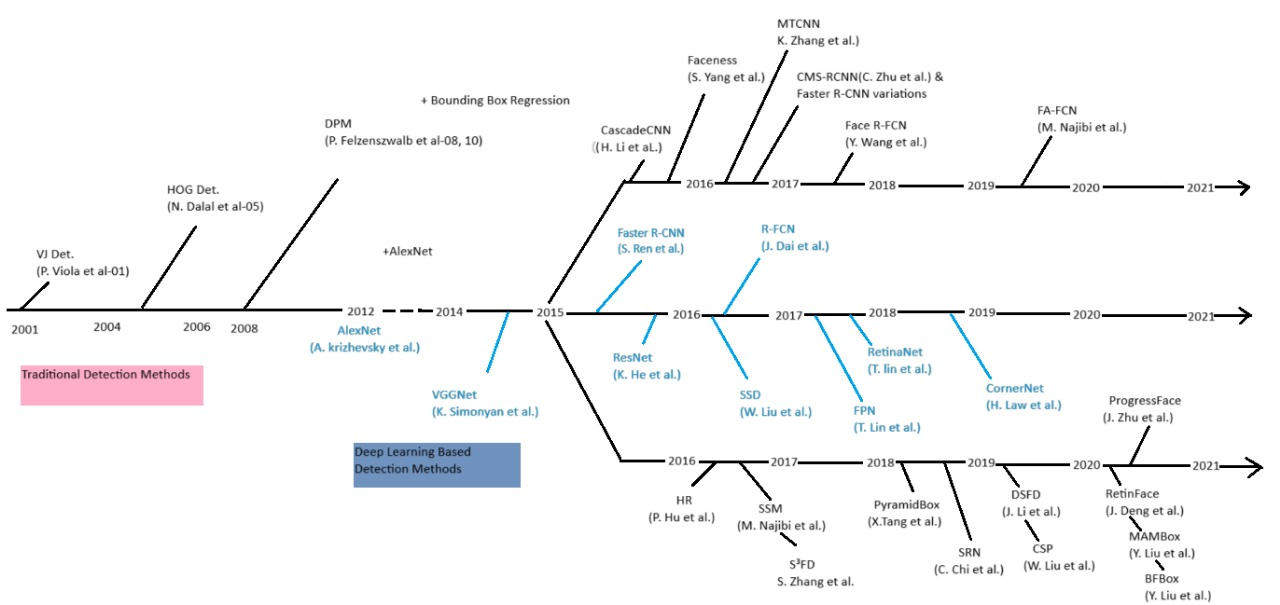
\includegraphics[width=\columnwidth]{assets/od-timeline.jpg}}
\caption{Object Detection and Face Detection Timeline Overview}
\label{od-timeline}
\end{figure}

Several methods and frameworks, like Viola-Jones \cite{sumanto_viola-jones_2022}, \cite{rani_face_2022}, HOG \cite{rani_face_2022}, MTCNN \cite{rani_face_2022}, MobileNet-SSD \cite{chan_face_2022}, and YOLO-Face \cite{wang_yolov5s-face_2022}, have been utilized to ensure consistent face detection in varying conditions. Once the face is extracted, recognition involves comparing faces within a certain range or threshold, with techniques like PCA and ICA used for accuracy. Lightweight model advancements, such as those based on lightweight models like GhostNet \cite{alansari_ghostfacenets_2023}, have also been explored to meet computational demands for lower end devices.

Authors in \cite{sumanto_viola-jones_2022} used ViolaJones method's on WIDER FACES dataset and achieved a 100\% success rate on detection in groups and meetings, while the previous approaches only managed the highest accuracy results were obtained at 90.9\% for facial images and 75.5\% for non-face images. While these approaches are good under controlled environments their accuracy decreases in uncontrolled environments. Exploring the challenges of detecting faces in uncontrolled environments with varying poses, addressing shortcomings caused by environmental factors, lighting conditions, and image quality authors in \cite{mahesh_smart_2022} proposed an 8-layer Alexnet Convolutional Neural Network (ACNN). By comparing ACNN with the Support Vector Machine (SVM), the research demonstrates that ACNN outperforms SVM, achieving a remarkable 96\% accuracy compared to SVM's 89\% in recognizing faces with varying poses.

Multitask-Net model proposed in \cite{viet_simultaneous_2021} overcomes the challenges of face detection and head pose estimation in digital images which is vital for applications like surveillance. The authors enhances head pose estimation accuracy by leveraging features from face detection and predicts head position and direction simultaneously, utilizing Rotation matrix vectors for face orientation representation to overcome limitations. The results showcase the model's high accuracy, comparable to state-of-the-art methods.

Addressing the issues of missed and false face detection Yongwang Wand et al. \cite{wang_yolov5s-face_2022} proposed a new model based on YOLOV5s by modifying the anchor box size using K-means clustering, embedding an SE attention module on the backbone of YOLOV5s and adding four-scale feature detection for small target faces. This new model gained 3.9\% in mAP and 4.0\% in Recall compared to YOLOV5s. In another paper by Aifian Adi Sufian et al. \cite{chan_face_2022} introduces a two-step face detection framework designed to reduce over-detection in face images and misdetection in non-face images. The method combines feature detection using SSD MobileNet V2 and a geometrical algorithm. When compared to leading algorithms the approach achieved a 91.5\% prediction accuracy. Although it didn't surpass MTCNN and Dlib in accuracy, it was superior in minimizing both over-detection and misdetection.

Farooq et al. \cite{farooq_hybrid_2021} highlights the challenges posed by variations in age, lighting, expressions, and image quality, especially for individuals with dark skin, where existing algorithms tend to perform poorly. To address this racial disparity in facial recognition technology, the authors presents a hybrid algorithm combining Gaussian Model and Explicit Rule Algorithm for skin detection. This innovative approach significantly improves the face detection accuracy for dark-skinned individuals by an impressive 89\%. This underscores the importance of diverse training datasets.

Night time video surveillance arising from varying environmental light conditions can lead to underexposed distant objects and overexposed nearby objects. To combat these issues, the authors in \cite{lu_fusion_2022} introduces the concept of a multi-intensity IR illuminator with periodically varying intensity. The MI3 database is established to assess object detectors in different scenes and illuminations. It evaluates human and face detectors, presenting satisfactory results for simple scenes and proposing a baseline approach for fusion among different illumination intensities.

Khalid M et al. \cite{hosny_privacy_2022} addresses the pressing need for privacy protection in surveillance videos, given the ubiquity of surveillance cameras in our lives. It focuses on safeguarding sensitive regions, particularly people's faces, within surveillance footage. The proposed method employs an object detector, YOLOv3 \cite{aziz_exploring_2020}, to identify the regions and subsequently applies a fast block scrambling technique for obfuscation. Encryption is then applied using secret keys generated from a chaotic logistic map. Notably, the method extends protection to the edges of detected regions to prevent sensitive information leakage. This approach offers practical and robust privacy protection for surveillance videos, ensuring the confidentiality of sensitive data and resilience against potential attacks.

While convolutional neural networks (CNNs) or other Deep learning based approaches have shown promise in face detection, their computational demands can be prohibitive, especially for CPU-based systems as it also adds to the computational complexity and thus requires good hardware which is often not the case with real time surveillance systems, the critical need for lightweight and efficient face detection methods without compromising accuracy was addressed by Muhamad Dwisnanto Putro et al \cite{putro_high_2021}. The authors introduces an optimized architecture, featuring a lightweight CNN with two key modules: a feature extraction backbone and a multilevel detector for accommodating scale variations in face detection. This innovative approach achieves state-of-the-art performance among CPU-based real-time detectors, running at an impressive 53 frames per second (FPS), while requiring fewer than one million parameters.
	\section{Face Tracking} \label{section:ft}
A face tracker is a computer vision system or algorithm designed to locate and follow a face in a sequence of frames or a video stream. The primary goal of face tracking is to maintain the identity of a face over time, regardless of facial movements, rotations, occlusions, or changes in facial expressions. Several technologies and algorithms, ranging from classical computer vision techniques to deep learning models, can be used in face tracking. A comprehensive survey of Siamese trackers in visual object tracking (a parent field of face tracking) was done by Milan Ondrasovic et al \cite{ondrasovic_siamese_2021}. Siamese trackers leverage deep learning and similarity learning for tracking objects in videos. They tackle challenges like scale and lighting variations, occlusion, and background clutter. According to authors recent trends involve using deeper backbones like ResNet \cite{aziz_exploring_2020}, multi-level feature fusion, and template updating strategies for improved performance. Cross-correlation with attention mechanisms has shown promise in achieving a balance between speed and accuracy.

Kim et al. \cite{kim_facial_2023} while developing a real time face recognition system used deepSORT as the tracking module. SORT (Simple Online and Realtime Tracking) is to provide a computationally efficient and straightforward method for tracking objects, especially in real-time scenarios. While SORT is computationally efficient and suitable for real-time scenarios, it's primarily designed for scenarios where the number of objects remains relatively constant, and there are minimal interactions or occlusions among objects. For more complex scenarios with numerous occlusions, interactions, and variable object counts, more sophisticated algorithms like DeepSORT (which augments SORT with deep learning-based features).

Multi-face tracking in unconstrained videos to identify and maintain the identities of multiple faces over time is important in real time face recognition system. An online multi-face tracking method was proposed in \cite{weng_online_2023} introduces a two-stage structure: detection alignment and detection association. It aligns face detections with body detections and matches these aligned detections with face or body features to form tracking trajectories. Experiments on benchmark databases demonstrate that utilizing both face and body information significantly enhances tracking performance compared to using only face data, making it competitive with or superior to other online tracking methods for multi-face tracking. Another approach introduces a cross-camera multi-face tracking system for video surveillance \cite{ren_cross-camera_2021}. It combines the Chinese Whisper face clustering algorithm and Double Triplet Networks (DTN) to accurately track pedestrians' faces across different cameras. Experimental results demonstrate its effectiveness, achieving a recognition accuracy of 99.51\% with the DTN MSML Batch OHNM Subspace FOCAL LOSS model. It addresses challenges like small target tracking and occlusion, offering a robust solution for efficient face tracking in surveillance scenarios.

Face tracking in crowded scenes presents a myriad of challenges, central to which is the issue of occlusions where faces are frequently obscured by other individuals or objects. Such environments often result in overlapping faces, making distinct identification and continuous tracking a daunting task. Authors in \cite{barquero_rank-based_2021} focused on enhancing video surveillance systems in crowded and unconstrained scenarios and introduces a novel tracklet reconnection strategy, utilizing rank-based face verification, to extend track lengths by up to 50\% compared to deep learning trackers. This constraint method also reduces identity mixing errors and improves completion rates.

The issues of video face clustering in the context of increasing facial appearance diversity was addressed by Vivek sharma et al. \cite{sharma_video_2020}. They introduced unsupervised methods for feature refinement using deep pre-trained face networks and self-supervised Siamese networks. Discriminative models like Track-supervised Siamese Network (TSiam) and Self-supervised Siamese Network (SSiam) are proposed alongside Variational Autoencoders (VAEs) as a strong generative model baseline. The methods are evaluated on challenging video face clustering datasets and outperform existing state-of-the-art techniques. According to authors the models are computationally efficient, making them suitable for diverse appearance datasets.
	\section{Face Recognition} \label{section:fr}
Facial recognition systems generally follow a three-step approach: face detection \ref{section:fd}, face tracking \ref{section:ft}, feature extraction, and identification or verification. While deep learning techniques have significantly improved facial recognition performance, achieving accuracy rates over 99\% on certain datasets, there are concerns about their real-world applicability, especially when recognizing individuals intent on avoiding detection \cite{kim_surveillance_2023}.

Face recognition starts with extracting the face area and its features, which can be a classification challenge to determine if the detected section is a face.

Facial recognition in videos can present ethical dilemmas, particularly in mistakenly identifying innocent bystanders. Most surveillance cameras record at 15 FPS due to storage constraints, but can capture at faster rates. Videos, which provide higher-dimensional data than static images, often give fragmented insights.

Authors in \cite{zhu_webface260m_2023} presents WebFace260M benchmark dataset, WebFace42M benchmark dataset and the Face Recognition Under Inference Time conStraint (FRUITS) protocol for comprehensive evaluation and addresses biased face recognition deployments, including masked and unbiased scenarios. 

Kim et al. \cite{kim_facial_2023} proposed a real-time Criminal Recognition system with 2 major update one is down sampling the input image for reducing the latency during the face detection, whereas high identification accuracy is maintained during the identification step by cropping the face regions from the original high-resolution images. Other update was introduction of Score Dictionary Identification where scores related to the identification results are accumulated for the face ID of each tracked face by creating a dictionary with the tracking ID as a key. The dictionary monitors the score such that when the score exceeds an arbitrary threshold, the system notifies parties of the identification result and transmits the appearance of the criminal.

\subsection{For Devices with limited Computational Power}

Alansari et al. \cite{alansari_ghostfacenets_2023} proposed a deep learning biometric models suitable for devices with limited memory and computational power by the introduction of Ghost modules marks a significant advancement. The model was named GhostFaceNets, lightweight face recognition models, are built upon GhostNetV1 and GhostNetV2, both rooted in Ghost modules. GhostFaceNets, when trained using the ArcFace loss on the refined MS-Celeb-1M dataset, showcased leading performance across benchmarks. They significantly boost efficiency in face verification compared to earlier top mobile CNNs. GhostFaceNets greatly improve efficiency for face verification tasks compared to previous SOTA mobile CNNs, making them suitable for deployment on devices with constrained memory and computational resources. In another such paper \cite{abuzneid_enhanced_2018} authors used back-propagation neural network (BPNN) and correlation-based feature extraction to improve face recognition accuracy. The proposed method achieves higher accuracy with reduced computational cost by generating a new set called the T-Dataset and using a local binary pattern histogram descriptor.

\subsection{Homogeneous Face Recognition}

Homogeneous Face Recognition generally refers to scenarios where the recognition system is designed to handle specific variations or challenges, such as age, pose, lighting, or expression.

With the advent of Covid-19 pandemic a new challenge for face recognition arise which was Masked Face Recognition. Given the global health circumstances since 2020 and the widespread adoption of face masks, masked face recognition has become a notable subfield within Homogeneous Face Recognition, addressing the unique challenges introduced by facial coverings.A masked face recognition algorithm with the combination of Convolutional Neural Network (CNN) and Support Vector Machine (SVM) was proposed by authors in \cite{9914874} where CNN is implemented to train the model, while SVM is used as a label classification method. Two benchmarked datasets, the Real World Masked Face Dataset (RMFD) and the Labelled Face in The Wild Simulated Masked Face Dataset (LFW-SMFD), are used in the experiments. The proposed method achieves a 98.39 percent true acceptance rate on RMFD and 94.29 percent on LFW-SMFD, demonstrating its practicality in recognizing unconstrained face images. Pedro Neto et al. \cite{pedro_neto_beyond_2022} accessed the performance of MFR algorithms was assessed on both masked and occluded face datasets. This assessment was again repeated using a top-performing occluded face recognition algorithm. Finally, to understand the broader context, the evaluation was again performed using algorithms intended for general face recognition. The authors evaluate several approaches for handling masks, including unmasking the input image, unmasking the template generated by a face recognition model, and using a model that is robust to masks.

Age significantly impacts face recognition due to the natural morphological changes that occur over time. Age-related factors can introduce intra-class variations that may pose challenges to recognition algorithms. Age-Invariant Model (AIM) \cite{zhao_towards_2022} was proposed for face recognition in the wild. The model performs cross-age face synthesis and recognition jointly. The AIM model achieves continuous face rejuvenation/aging with photorealistic and identity-preserving properties, without the need for paired data or the true age of testing samples.

\subsection{Heterogeneous Face Recognition}

One other field of face recognition is Heterogeneous Face Recognition (HFR) which refers to the task of matching faces across different domains or modalities. It involves matching a near-infrared (NIR) facial image with a visible light facial image, a sketch of a face with a photographic image, or a thermal image of a face with a regular visible spectrum image etc. A Dual variational generation (DVG-Face) \cite{fu_dvg-face_2022} framework to tackle the heterogeneous face recognition (HFR) problem. It formulates HFR as a dual generation problem and designs a dual variational generator to learn the joint distribution of paired heterogeneous images. A pairwise identity preserving loss is imposed on the generated paired heterogeneous images to ensure their identity consistency. The generated paired heterogeneous images are used to train the HFR network via a contrastive learning mechanism, which yields both domain-invariant and discriminative embedding features. DVG-Face outperforms state-of-the-art methods on seven challenging databases belonging to five HFR tasks, including NIR-VIS, Sketch-Photo, Profile-Frontal Photo, Thermal-VIS, and ID-Camera.
Decheng Liu et al. \cite{liu_heterogeneous_2022} proposed approach with three components, a Graph Convolutional Autoencoder (GCA) for encoding 3D faces into latent representations, a Generative Adversarial Network (GAN) for translating the latent representations of expressive faces into those of neutral faces, and an identity recognition sub-network that utilizes the neutralized latent representations for 3D face recognition. This has practical implications in the field of 3D face recognition and expression neutralization. It offers a method to generate realistic 3D faces with neutral expressions while predicting their identities.
Face Synthesis with Identity-Attribute Disentanglement (FSIAD) \cite{yang_heterogeneous_2022} for Heterogeneous Face Recognition involves two main steps: identity-attribute disentanglement (IAD) and face synthesis module (FSM). Face images are separated into identity-related representations and identity-unrelated representations (attributes) to decrease the correlation between identities and attributes in the IAD step and the FSM is then used to generate a large number of images with stochastic combinations of disentangled identities and attributes, enriching the attribute diversity of synthetic images.

	\section{Datasets} \label{section:datasets}

Datasets play a crucial role in the development, training, and evaluation of face detection and recognition systems. They provide researchers with rich resources such as transfer learning where large face datasets can be used to pre-train models, which can then be fine-tuned on smaller, task-specific datasets is often results in better performance than training on the smaller dataset alone.

Requirements of a good dataset are as follows:

\begin{enumerate}
    \item \textbf{Diversity}: The dataset should encompass a wide variety of facial features, expressions, angles, and occlusions. This ensures that the trained models generalize well to real-world scenarios.

    \item \textbf{High Quality Images}: Images should be of high resolution and clarity. Blurry or low-quality images can hinder the performance of detection or recognition systems.

    \item \textbf{Varied Lighting Conditions}: It should include faces under different lighting conditions - from well-lit to poorly lit scenarios - to challenge and enhance the robustness of algorithms.

    \item \textbf{Age Variability}: Faces from different age groups, ranging from infants to the elderly, should be represented to ensure age-invariance in recognition.

    \item \textbf{Demographic Diversity}: A balanced representation of various ethnicities, genders, and backgrounds is essential to prevent biases in the resulting models.

    \item \textbf{Annotations}: Precise annotations, including bounding boxes for detection and identity labels for recognition, are crucial.

    \item \textbf{Temporal Data}: For video-based recognition systems, the dataset should include video sequences to account for temporal variations and movements.

    \item \textbf{Real-world Scenarios}: Inclusion of "in-the-wild" images or videos where faces are naturally occluded, or in varied expressions and postures, simulates real-world challenges.

    \item \textbf{Scalability}: A good dataset should be large enough to train deep learning models, which often require vast amounts of data.

    \item \textbf{Consent and Ethics}: All data should be collected with proper consent, ensuring the privacy and rights of the individuals are respected.
\end{enumerate}



WebFace260M benchmark \cite{zhu_webface260m_2023}, an ultra-large-scale dataset comprising 4 million identities and 260 million faces was introduced to bridge the data gap between academia and industry. The dataset was still refined by employing the Cleaning Automatically by Self-Training (CAST) pipeline,into WebFace42M, with 2 million identities and 42 million faces. The benchmark and cleaned dataset facilitate efficient model training, resulting in improved face recognition performance and potential solutions for bias mitigation and privacy concerns in the field. The benchmark and cleaned dataset facilitate efficient model training, resulting in improved face recognition performance and potential solutions for bias mitigation and privacy concerns in the field.

Zhongyuan Wang et al. \cite{wang_masked_2023} proposes three types of masked face datasets: Masked Face Detection Dataset (MFDD), Real-world Masked Face Recognition Dataset (RMFRD), and Simulated Masked Face Recognition Dataset (SMFRD). The Real-world Masked Face Recognition Dataset (RMFRD) is claimed to be the world's largest real-world masked face dataset by the authors. Although the details of the specific methods used in developing the datasets are not mentioned in the provided sources. DVG-Face framework \cite{fu_dvg-face_2022} was evaluated on seven challenging databases belonging to five HFR tasks, including NIR-VIS, Sketch-Photo, Profile-Frontal Photo, Thermal-VIS, and ID-Camera, and achieves superior performances over state-of-the-art methods and outperforms them. Zhao et al. \cite{zhao_towards_2022} curated a new large-scale Cross-Age Face Recognition (CAFR) benchmark dataset to facilitate research in age-invariant face recognition for their AIM model. Extensive experiments are conducted on the CAFR dataset and other cross-age datasets (MORPH, CACD, FG-NET) to demonstrate the superiority of the proposed AIM model over existing techniques. The AIM model is further benchmarked on unconstrained face recognition datasets (YTF, IJB-C) to verify its generalization ability in recognizing faces in the wild.

Authors in \cite{abuzneid_enhanced_2018} used 3 datasets YALE and AT\&T for testing the proposed framework and evaluated their method on the LFW dataset, which is a state-of-the-art benchmark dataset for face recognition.

Detection in a controlled environment often leads to good results but when the model is deployed in an uncontrolled environment with noise, occlusion, extrnal lighting, makeups etc often referred as ``in the wild" then the accuracy drops. But there are dataset with these kinds of images. One such dataset is the WIDER FACE dataset, which is used as a training dataset for the CNN based lightweight detector in \cite{putro_high_2021}. It contains 32,203 images, with 12,800 images specifically used for training the detector. Augmentation techniques are applied to enrich the training data and prevent overfitting during the training process. The second dataset is the PASCAL face dataset \cite{putro_high_2021}, which consists of 851 images with 1335 labelled faces. This dataset is a subset of the PASCAL VOC dataset and includes variations in pose and background, both indoor and outdoor.

Datasets like VGGFace2 and MS-Celeb-1M, which primarily contain data from young, facially beautiful celebrities with makeup, are biased in terms of age and facial appearance, leading to potential performance issues when using pretrained models from these datasets on different audiences \cite{wanyonyi_open-source_2022}.

Tables \ref{det-ds} and \ref{rec-ds} contains a list of popular publicly available datasets found in the literature survey:

\begin{table}[htbp]
\caption{Detection Datasets}
\begin{center}
\begin{tabularx}{\columnwidth}{|X|c|X|}
\hline
\textbf{Dataset} & \textbf{Year}& \textbf{Size} \\
\hline
VGGFace2 \cite{kim_face_2022} & 2018 & 3.31 million images of 9,131 subjects \\
\hline
WIDER Face \cite{kim_face_2022} & 2016 & 32,203 images with 393,703 annotated face bounding boxes \\
\hline
VGGFace2 \cite{kim_face_2022} & 2018 & 3.31 million images of 9,131 subjects \\
\hline
PASCAL Face \cite{feng_detect_2022} & 2012 & 1,335 faces from 851 images \\
\hline
\end{tabularx}
\label{det-ds}
\end{center}
\end{table}
    
    
\begin{table}[htbp]
\caption{Recognition Datasets}
\begin{center}
\begin{tabularx}{\columnwidth}{|X|c|X|}
\hline
\textbf{Dataset} & \textbf{Year}& \textbf{Size} \\
\hline
MS-Celeb-1M \cite{wanyonyi_open-source_2022} & 2016 & 10 million images of 100,000 celebrities \\
\hline
LFW \cite{kim_face_2022} & 2007 & 13,000 images of 5,749 distinct individuals \\
\hline
CASIA NIR-VIS 2.0 \cite{liu_heterogeneous_2022} & 2007 & 17,580 images from 725 subjects \\
\hline
ChokePoint \cite{barquero_rank-based_2021} & 2011 & 54 video sequences captured from 6 different camera views \\
\hline
\end{tabularx}
\label{rec-ds}
\end{center}
\end{table}
	\section{Conclusion} \label{section:conclusion}

In this survey, we have traversed the multifaceted landscape of facial recognition. We delved deep into the core challenges posed by occlusions, crowd dynamics, and ever-shifting backgrounds, each of which has the potential to compromise recognition accuracy.

Our exploration spanned from the foundational algorithms of face detection and recognition to the latest advancements tailored to address the nuances of real-world scenarios. We analysed various methods, ranging from classic computer vision techniques to the pinnacle of deep learning architectures, shedding light on their strengths, weaknesses, and applicability. The role of datasets, as a bedrock for training, validating, and benchmarking these algorithms, was emphasized, emphasizing their significance in shaping the field's trajectory.

Yet, as with any evolving technology, the journey of refining and perfecting real-time face recognition is ongoing. The dynamic interplay of technical challenges, evolving societal contexts (like the widespread adoption of masks), and the ever-present imperative of ethical considerations ensures that this domain will remain at the forefront of research for years to come.

This survey, while comprehensive, is but a snapshot of the current state of affairs. As the field progresses, new challenges will emerge, and novel solutions will be conceived. Nevertheless, our hope is that this work serves as a robust foundation and reference point, catalysing further innovations and guiding researchers and practitioners alike in their endeavours to harness the full potential of real-time face recognition, especially in the service of public safety and law enforcement.

	\bibliographystyle{IEEEtranN}
\bibliography{
	components/refs/settings.bib,
	components/refs/intro.bib,
	components/refs/fr.bib,
	components/refs/all.bib
}

\end{document}
